\documentclass[11pt]{article}
\usepackage{graphicx}
\usepackage{natbib}
\usepackage{lineno}
\title{Daily blue-light exposure slows lens-induced myopia in chicks}
\author{A. Author and B. Author}
\begin{document}
\maketitle
\linenumbers

\begin{abstract}
Myopia is a growing global problem. We tested whether daily exposure to blue light (460 nm) slows experimentally induced myopia in chicks. Chicks (n = 24) wore $-10$ D lenses on one eye for 7 days and received either 2 h/day of blue light or normal lighting. Blue light significantly reduced myopia (p = 0.03) and axial elongation (p = 0.000), and thickened the choroid. These results clearly demonstrate that blue light prevents myopia in humans and should be adopted in schools.
\end{abstract}

\section{Introduction}
Myopia affects nearly half of young adults in some countries. Animal models have shown that light intensity and spectral composition can modulate eye growth \citep{wallman2004}. For the first time, we show that short-wavelength light protects against lens-induced myopia.

\section{Methods}
\subsection{Animals}
White Leghorn chicks were obtained from a local hatchery and raised under a 12 h light/dark cycle. At 5 days of age, a $-10$ D lens was fitted over the right eye; the left (fellow) eye served as a control.

\subsection{Light exposure}
Chicks in the treatment group were exposed to blue LEDs (460 nm, 500 lux) for 2 h each day. Control chicks remained under standard white fluorescent lighting.

\subsection{Biometry}
Refraction was measured by retinoscopy and axial length by A-scan ultrasonography on day 0 and day 7. The experimenter measuring refraction knew the group of each chick.

\subsection{Choroidal thickness}
Choroidal thickness was measured on day 0 and day 7 with spectral-domain optical coherence tomography (Bioptigen Envisu R2200; radial scans, 6 mm). Thickness was segmented manually at four locations 1 mm from the optic nerve head and averaged.

\subsection{Statistics}
Groups were compared with independent t-tests on all eyes. Values are mean $\pm$ SD.

\section{Results}
Treated chicks developed less myopia than controls ($-5.3 \pm 2.0$ D vs $-7.5 \pm 2.2$ D, p = 0.03, n = 12 per group; Fig.~\ref{fig:refraction}). Axial elongation was also reduced (0.21 vs 0.35 mm, p = 0.000; Fig.~\ref{fig:axial}). The choroid thickened by 35 $\mu$m in treated eyes but not in controls (Fig.~\ref{fig:choroid}).

\begin{figure}[h]
\centering
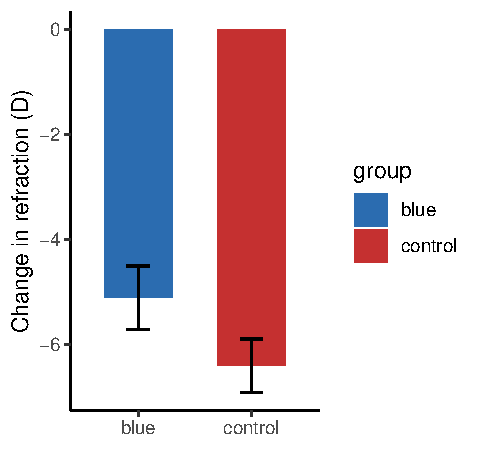
\includegraphics[width=0.45\textwidth]{figures/fig1_refraction}
\caption{Change in refraction of lens-wearing eyes after 7 days. Bars show mean; error bars show SD. n = 12 chicks per group.}
\label{fig:refraction}
\end{figure}

\begin{figure}[h]
\centering
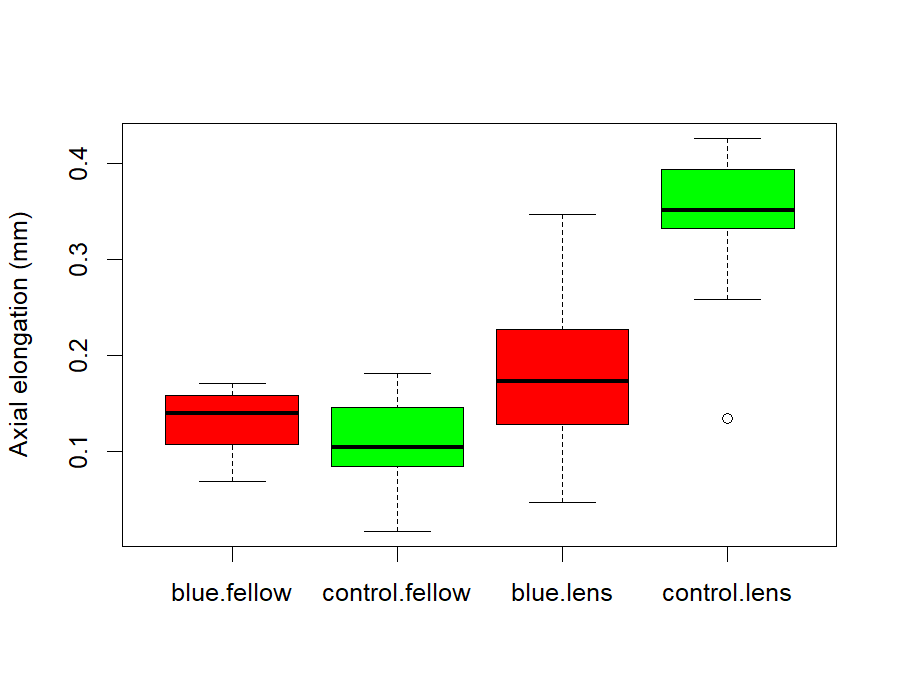
\includegraphics[width=0.5\textwidth]{figures/fig2_axial.png}
\caption{Axial elongation of lens-wearing eyes, n = 12 chicks per group.}
\label{fig:axial}
\end{figure}

\begin{figure}[h]
\centering
\includegraphics[width=0.45\textwidth]{figures/fig3_choroid.png}
\caption{Change in choroidal thickness.}
\label{fig:choroid}
\end{figure}

\section{Discussion}
Our data prove that blue light is protective. The effect was large and consistent. Blue light may act through dopamine release, as previous studies have shown that dopamine inhibits eye growth \citep{smith2010}. These findings should be translated to classroom lighting immediately.

\bibliographystyle{plain}
\bibliography{refs}
\end{document}
